\section{Potenziometro a filo avvolto}\label{sec:filoavvolto}
Si tratta di un filo di lega metallica con resistività e dimensioni
stabili che viene avvolto lungo un cilindro rigido; un cursore,
anch'esso metallico, viene poso sopra al cilindro di modo che possa
fare contatto sul filo avvolto e sarà proprio su questo cursore che
verrà prelevata la tensione di riferimento per il campionamento. In
figura \ref{fig:filoavvolto} è possibile vederne una
rappresentazione schematica, mentre in figura \ref{fig:potenziometro}
la rappresentazione circuitale.

\begin{figure}[htbp]
	\centering
	\includegraphics[scale=0.5]
			{img/filoavvolto.png}
	\caption{Potenziometro a filo avvolto\label{fig:filoavvolto}}
\end{figure}

\begin{figure}[htbp]
	\centering
	\includegraphics[scale=0.5]
			{img/potenziometro.pdf}
	\caption{Potenziometro\label{fig:potenziometro}}
\end{figure}

Per ricavare il valore della tensione in uscita V basta applicare la
regola del partitore di tensione, immaginando che le due resistenze
siano rappresentate: una dalla parte alla sinistra del cursore (sulla
quale si preleva la misura della tensione) e l'altra dalla parte alla
destra del cursore come in figura \ref{fig:potenziometroequiv}.

\begin{figure}[htbp]
	\centering
	\includegraphics[scale=0.5]
			{img/potenziometro-equiv.pdf}
	\caption{Circuito equivalente
per il potenziometro\label{fig:potenziometroequiv}}
\end{figure}

Il problema è ora quantificare il valore di queste
due resistenze e metterlo in relazione con con lo spostamento $X$ del
cursore rispetto all'inizio (cioè quando il cursore è tutto a
sinistra). Ora indichiamo con $L$ la lunghezza del potenziometro e
calcoliamo $V$:

\[ R = \frac{L}{S}\rho \rightarrow R_1=\frac{L-S}{S}\rho,
R_2=\frac{S}{S}\rho \]
\[V=E\frac{R_2}{R_1+R_2}=E\frac{\rho\frac{X}{S}}{\rho\frac{L-X}{S}
+ \rho\frac{X}{S}}= E \frac{X}{L}\]

Da qui la relazione che lega $V$ con $X$:

	\[\frac{X}{L} = \frac{V}{E}\]

\subsection{Vantaggi}
Il primo vantaggio è la linearità: la resistività uniforme del cavo
permette una distribuzione di potenziale che è lineare nello spazio.
Un secondo vantaggio, è la possibilità di ottenere un segnale
elettrico di ampiezza desiderato. Il trasduttore è insensibile alla
variazione di temperatura se questa avviene uniformemente su l'intero
trasduttore.
\subsection{Svantaggi}
La risoluzione limitata dovuto allo spazio vuoto fra due avvolgimenti
del filo metallico, inoltre in questo spazio si può perdere la misura.
La vita media breve a causa dell'usura generata dal movimento del
cursore e, infine, la forza necessaria per vincere l'attrito generato
dal movimento del contatto provoca un'alterazione del sistema sotto
misura, quindi possono esserci possibili isteresi.

\section{Potenziometro a strato di carbonio}\label{sec:potcarbonio}
Il funzionamento è del tutto analogo a quello del potenziometro a filo
avvolto\ref{sec:filoavvolto} con la differenza che a fornire la
resistenza c'è ora uno strato di carbonio sul quale va a posizionarsi
il cursore.

\begin{figure}[htbp]
	\centering
	\includegraphics[scale=0.5]
			{img/potenziometro-carbonio.pdf}
	\caption{Potenziometro a
strato di carbonio\label{fig:potenziometro-carbonio}}
\end{figure}

Il vantaggio introdotto è che ora la risoluzione non è più
a scalino ma è lineare lontano dagli estremi, lo svantaggio invece è
la vita molto breve dovuto al consumo dello strato di carbonio causato
dallo sfregamento del cursore su di esso.

\section{Potenziometro elettro-ottico
(fotopotenziometro)}\label{sec:elettrottico}
Essendo un potenziometro, il suo comportamento è analogo a quello
visto per il potenziometro a filo avvolto\ref{sec:filoavvolto}, cambia
solo il modo in cui viene realizzato. La realizzazione di un
potenziometro elettro-ottico prevede di unire un film resistivo con
una striscia di materiale foto-conduttore e del materiale conduttore.

\begin{figure}[htbp]
	\centering
	\includegraphics[scale=0.5]
			{img/fotopotenziometro.png}
	\caption{Foto-potenziometro\label{fig:fotopotenziometro}}
\end{figure}

A questo punto sopra a questi tre elementi viene posta una lamina
tagliata. Attraverso la lamina viene fatta passare la luce che farà
passare la corrente nel punto in cui il materiale fotoconduttore è
illuminato permettendo così di prelevare la tensione V sul materiale
conduttore.

\subsection{Vantaggi}
Il principale vantaggio è l'assenza di contati meccanici striscianti
e di conseguenza una vita più lunga del trasduttore. Questo tipo di
potenziometro offre una maggiore risoluzione.
\subsection{Svantaggi}
Questo tipo di potenziometro garantisce una linearità inferiore,
inoltre è molto più complesso, quindi costoso, da realizzare.
Richiede il buio totale in quanto le infiltrazioni di luce esterna
potrebbero introdurre errori.

\section{Trasduttore capacitivo}\label{sec:potcapacitivo}
Esso è costituito da tre armature di metallo di cui due fisse ed
allineate e una mobile che si muove sopra le altre due creando così
due capacità differenti che variano a seconda dell'area dell'armatura
mobile che copre una delle due armature. In figura
\ref{fig:potcapacitivo} una rappresentazione schematica.

\begin{figure}[htbp]
	\centering
	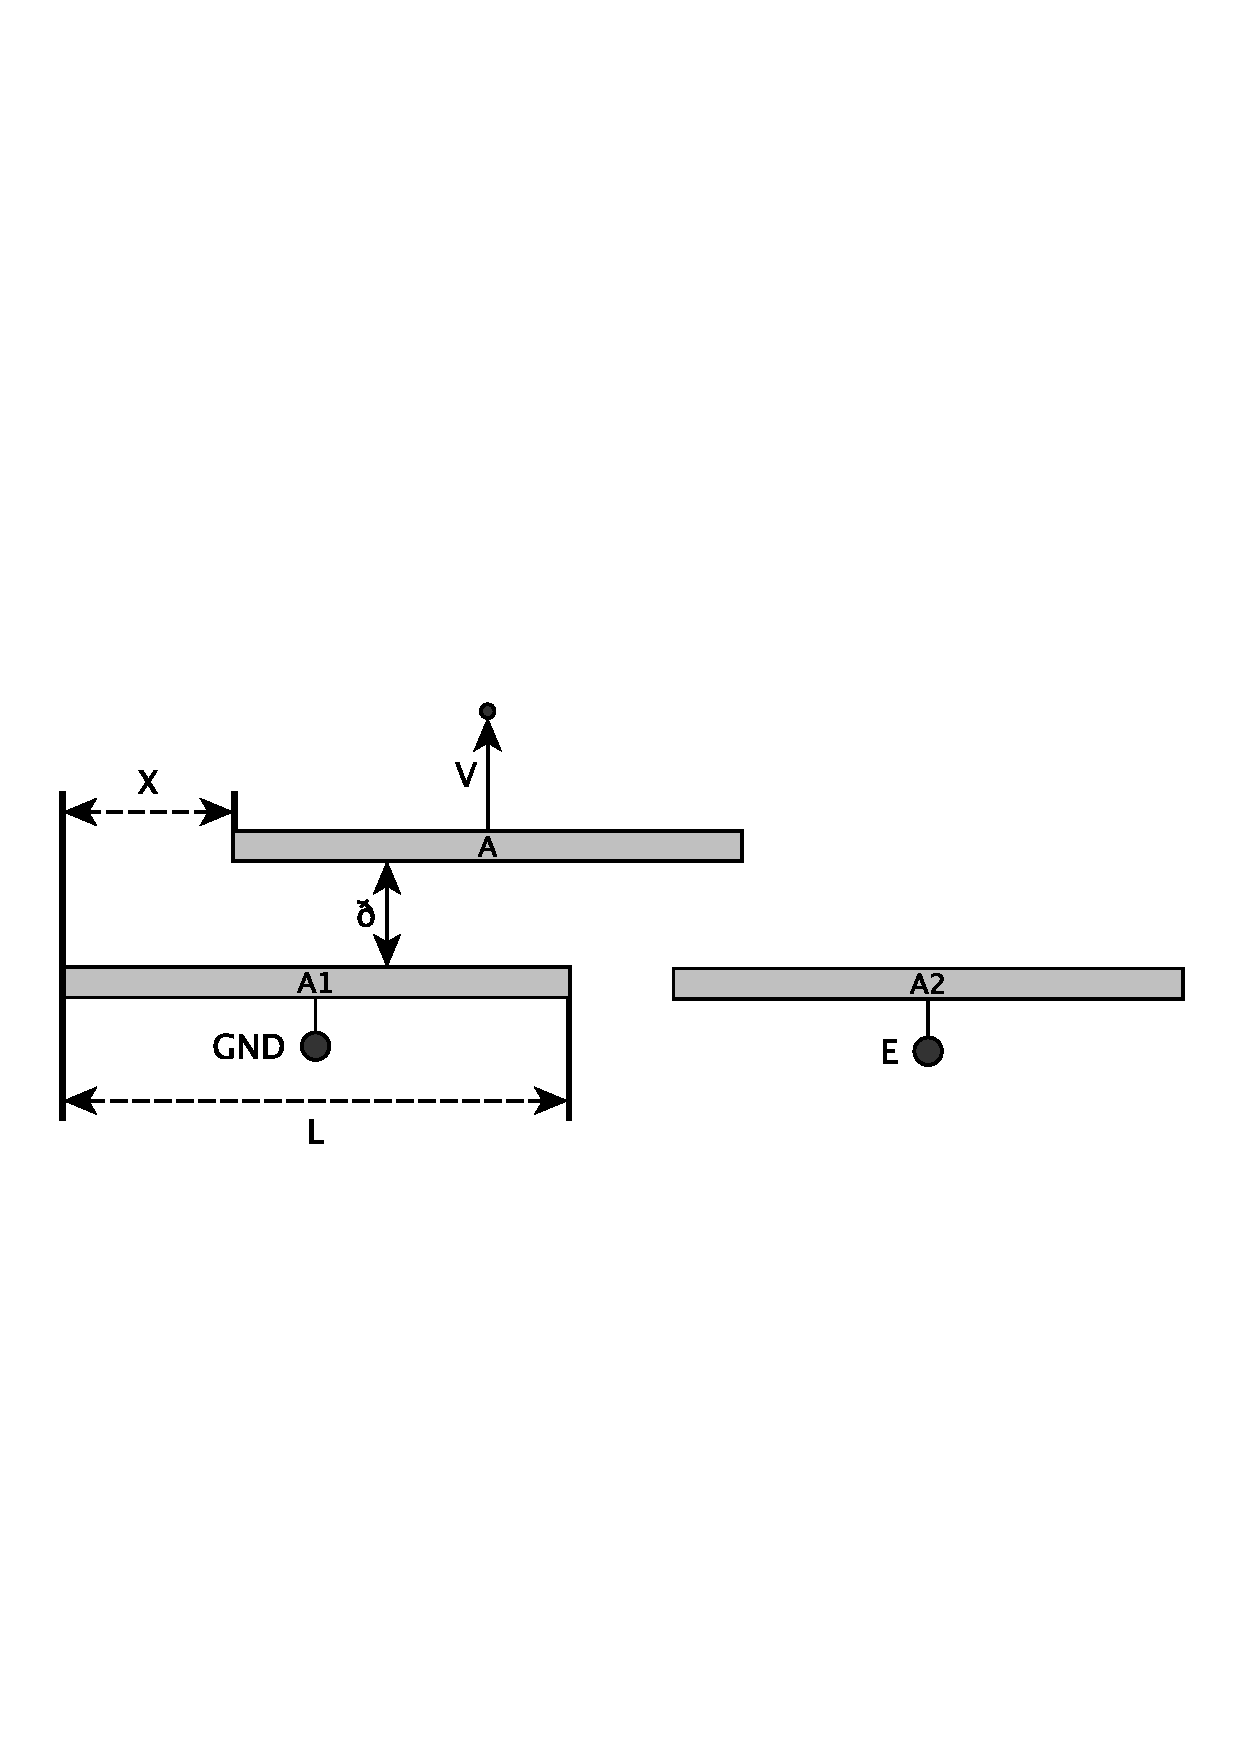
\includegraphics[scale=0.5]{img/potenziometro-capacitivo.pdf}
	\caption{Potenziometro capacitivo\label{fig:potcapacitivo}}
\end{figure}

In questo modo sempre col partitore di tensione possiamo misurare lo
spostamento. In figura \ref{fig:potcapacitivoequiv} il circuito
equivalente.

\begin{figure}[htbp]
	\centering
	\includegraphics[scale=0.5]
			{img/potenziometro-capacitivo-equiv.pdf}
	\caption{Circuito equivalente
del trasduttore capacitivo\label{fig:potcapacitivoequiv}}
\end{figure}

Le capacità $C_1$ e $C_2$ sono le capacità che si vengono a creare
dalla sovrapposizione delle armature $A_1$ e $A_2$ con l'armatura $A$.
$H$ indica la profondità dell'armatura.

	\[
	C_1=\frac{H (L-x)}{\delta}\varepsilon_0,
	C_2 =\frac{Hx}{\delta}\varepsilon_0
	\]
	\[
	V=E\frac{\frac{1}{sC_1}}{\frac{1}{sC_1}+\frac{1}{sC_2}}
	 =E\frac{C_2}{C_1+C_2}
	 =E\frac{\frac{Hx}{\delta}\varepsilon_0}
		{\frac{Hx}{\delta}\varepsilon_0+
				\frac{H(L-x)}{\delta}\varepsilon_0}
	 =E\frac{x}{L}
	\]

\subsection{Vantaggi}
I vantaggi sono gli stessi del potenziometro
elettro-ottico\ref{sec:elettrottico}
\subsection{Svantaggi}
Questo trasduttore soffre di scarsa linearità agli estremi; inoltre
si hanno problemi di carico inquanto l'impedenza del condensatore è
elevata, questo suggerisce l'utilizzo di un buffer ad alta
impedenza d'ingresso. Per ultimo, quando si lavora in
tensione alternata si rende necessario un circuito raddrizzatore a
valle del potenziometro.

\subsection{Variazione di impedenza}
Un alternativa è quella di usare un trasduttore di posizione
capacitivo a variazione d'impedenza, costruito come due cilindri che
si inseriscono uno dentro l'altro e muovendoli varia la capacità come
$C=KX$ e quindi anche l'impedenza.

\begin{figure}[htbp]
	\centering
	\includegraphics[scale=0.5]
			{img/potenziometro-capacitivo-2.png}
	\caption{Potenziometro
capacitivo alternativo\label{fig:potcapacitivoalt}}
\end{figure}

\section{Trasformatore differenziale}
La trasduzione si basa sul principio della mutua induttanza variabile:
per realizzare ciò si utilizza un avvolgimento primario e due
avvolgimenti secondari di accoppiamento. L'accoppiamento avviene
tramite un cilindro ferromagnetico di sezione $S$ e lunghezza $L$ che
si muove fra il primario e il secondario.

\begin{figure}[htbp]
	\centering
	\includegraphics[scale=0.5]
			{img/trasformatore-differenziale.png}
	\caption{Trasformatore differenziale\label{fig:trasdiff}}
\end{figure}

Le due induttanze secondarie sono in serie ma in opposizione di fase,
ne risulta quindi che $V_{out}=E_1-E_2$. La direzione dello
spostamento si deduce a seconda che $V_out$ sia in fase con $e$ o
meno. Indichiamo con $N_1$ il numero di spire coperte dal cilindro sul
primo solenoide e $N_2$ il numero di spire coperte dal cilindro sul
secondo, mentre con $B$ il campo magnetico del cilindro
ferromagnetico. Definiamo quindi il flusso di $B$ attraverso ad una
singola spira (anche lei di sezione $S$) e quindi il flusso sui
solenoidi 1 e 2:

	\[\phi=BS\]
	\[\phi_1=\phi N_1, \phi_2=\phi N_2 \]

A questo punto possiamo definire la forza elettro motrice sui due
solenoidi:

	\[E_1=j\omega\phi_1, E_2=j\omega\phi_2 \]

La tensione in uscita sarà quindi data da:

	\[V_out = E_1 - E_2 = j\omega\phi[N_1 - N_2]\]

Prendendo come posizione di riferimento dello spostamento, il punto
centrale fra i due secondari, avremo che in condizione di riposo il
cilindro compre metà spire del primo solenoide e metà del secondo,
quindi:

	\[N_1 = [\frac{L}{2}+X]n, N_1 = [\frac{L}{2}-X]n\]

dove $n$ è la densità di spire dei solenoidi. Da questa
considerazione ne consegue che:

	\[V_out=j\omega\phi 2nX\]

L'uso di questo trasduttore è consigliato a base frequenze perché vi
è un'impedenza in uscita minore ($j\omega Z_L$).
Da notare che avviene un'inversione di fase per spostamenti negativi;
in figura \ref{fig:trasdifffase} la rappresentazione del segnale in
uscita.

\begin{figure}[htbp]
	\centering
	\includegraphics[scale=0.5]
			{img/trasformatore-differenziale-fase.png}
	\caption{Segnale in uscita da un trasformatore
differenziale\label{fig:trasdifffase}}
\end{figure}

\section{Trasduttore ad induttanza variabile}
Vengono posti in vicinanza due pezzi di materiale ferromagnetico, uno
a ferro di cavallo e l'altro a forma di barretta; quest'ultima è
mobile, quindi è possibile avvicinarla o allontanarla misurando così
lo spostamento.

\begin{figure}[htbp]
	\centering
	\includegraphics[scale=0.5]
			{img/induttanza-variabile.png}
	\caption{Trasduttore ad induttanza
variabile\label{fig:trasdifffase}}
\end{figure}

Possiamo ora calcolare la riluttanza del circuito ferromagnetico;
teniamo conto però solo dei tratti $L_5$ ed $L_3$ in quanto gli unici
significativi per la determinazione della distanza ($S$ indica la
sezione del ramo e $\mu$ la permeabilità, $\mu_0$ la permeabilità
del vuoto).

	\[\Re=\sum_i{\frac{L_i}{S_im_i}}\]
	\[\Re=\frac{L_2}{S_2\mu_3} + \frac{L_5}{S_5\mu_5}
	     =2\frac{X}{S\mu_0}\]

La riluttanza può essere misurata avvolgendo un certo numero di spire
attorno al ramo $L_1$; le spire vengono disposte con una densità $n$.
Ne risulta che l'induttanza corrisponde a:

	\[
	L=\frac{n\phi}{I}
	 =\frac{\frac{n^2i}{\Re}}{i}
	 =\frac{n^2}{\Re}
	 =\frac{n^2S\mu_0}{2X}
	\]
Da qui possiamo ricavare l'ammettenza:

	\[Y=Z^{-1}=\frac{1}{\omega L}=\frac{2X}{\omega n^2S\mu_0}\]

Ne consegue che alimentando il circuito e misurando la
corrente $I=VY$, questa varierà al variare della distanza $X$

\subsection{Vantaggi}
La possibilità di regolare l'impedenza variando il numero di
spire avvolte sul materiale ferromagnetico (su $L_1$ per la
precisione) e la possibilità di fare misure di induttanza a frequenze
relativamente basse.
\subsection{Svantaggi}
La linearità peggiora più ci si allontana dal nucleo e
problemi di misura in alternata. Inoltre in corrente alternata abbiamo
problemi di misura.

\subsection{Trasduttore ad induttanza variabile alternativo}
Per colmare il difetto della linearità è possibile porre la barra
ferromagnetica fra due ferri di cavallo di modo che se peggiora
allontanandosi da uno, migliora avvicinandosi all'altro.

\begin{figure}[htbp]
	\centering
	\includegraphics[scale=0.5]
			{img/induttanza-variabile-2.png}
	\caption{Trasduttore ad induttanza
variabile alternativo\label{fig:trasdifffase}}
\end{figure}